\documentclass{article} 
%% Look like nroff
%% Sans serif font, virtually no line spacing, small titles, small margins, no page numbers
\renewcommand{\familydefault}{\sfdefault}
\linespread{.8}
\usepackage{titlesec}
\titlelabel{\thetitle. }
\titleformat*{\section}{\bf}
\titleformat*{\subsection}{\bf}
\pagenumbering{gobble}

\usepackage{amsmath} 
\usepackage{hyperref} 
\usepackage{fullpage}
\usepackage[a4paper,margin=2cm]{geometry}
\usepackage{graphics}


\title{WIP: Nix Reborn}
\author{Minnich, Ron\\
	\texttt{rminnich@gmail.com}
	\and
	Laronde, Thierry\\
	\texttt{tlaronde@kergis.com}
	\and
	Lalonde, Paul\\
	\texttt{plalonde@acm.org}
	}
\date{\today} 

\begin{document} 
\newcommand{\PAL}[1]{{\em PAL: #1}}
\maketitle 
\abstract
Nix is a derivative of the Plan 9 operating system\cite{Pike:1990:PBLa}, focusing on many-core performance. It allows tasks to be assigned to a particular core after which
that core will not be interrupted or assigned more work until the process yields cooperatively.  This leads to a very low overhead for compute on that core.
The original implementation of Nix \cite{Ballesteros2012} was done as a full fork of the Plan9 environment.  Since then hardware has continued to evolve and
that branch is no longer a viable system.
Futher, 9front has emerged as the Plan9 distribution that ``just works'', with the addition of many device drivers, kernel structure improvements, improved
 boot method support, and many useful userland changes.
This paper presents a new port of the Nix ideas into 9front.  The changes are mostly non-invasive, limited to a dozen or so files.  Only one significant change is required to the Mach structure for tracking the scheduling class of a core.

\section{Introduction}
Nix originated in 2011, a first attempt at examining manycore OS design starting from Plan9.
The result was achieved in about one month of effort with a small team\cite{Ballesteros2012}.  This is also a tribute to the simplicity of the Plan9
architecture. % composed of: Enrique Soriano, Charles Forsyth, Jim McKie, Francisco J. Ballesteros, Noah Evans, Gorka Guardiola and Ron Minnich.
The results were promising but the effort faltered, due to funding, Plan9 licensing constraints, and modern hardware support.

When the processor industry hit a limit when trying to improve efficiency by inceasing frequency improvements had to come from
another source: increasing the number of cores, enabling parallel processing.
But operating systems have lagged behind.
Though all modern operating systems support multi-core systems, no significant modifications to the timesharing model have occurred.
As multi-core machines gain more and more cores --- now reaching into the thousands in some cases \cite{Ditzel2022} --- the question arrises if it remains sensible to treat all cores equally in terms of distribution of user workloads and operating system support work.

Nix was the answer to a question: what if, rather than having CPUs with thousands of cores, each running a kernel and programs; we had, e.g., 32 kernel-capable cores and 1024 cores that could only run programs?
What would that system look like? 

We learned that "user-only" cores would be hard to implement; it seems we also need some minimal capability to handle a trap. We also learned that it is valuable to have shared memory, which makes it possible to easily switch a program from "running on an application core" to "running on a kernel core" -- without this, Nix is much harder to write in a transparent way.
Finally, we learned that "it always works" is a key idea -- Nix apps designed to work on application cores should always work even if they can only run on kernel cores; and using application cores should be so easy as to be invisible.
Users should never need to think about where their code will work, and where it will not: it should just work.
As a result, Nix is very transparent to the user.
Nix added one new system call -- execac -- which allows a user to indicate "whatever core is available" or to pick the core to use.
Standard exec is layered over execac.
Nix also added an rfork option to allow processes to easily switch to running on an application core.
Nix also minimally extended rc to allow users to pick a core to run a command on, or a set of cores in a pipeline, one core per pipe element [this code is lost].
With these small changes, Nix became an easy and fast environment in which to run with differentiated cores.

This naturally leads to the modern question: how do we write an operating environment for systems of "differentiated cores", such as x86 CPUs with "performance" cores and "power efficient" cores; or Esperanto with its Maxions and Minions?
It seems Nix still has an answer to questions of today.

\subsection{Modern Hardware}
The environment in which Plan 9 now runs has changed.
9front now provides good support for a range of common hardware.
CPUs have evolved to where even a commodity PC solutions offer eight to 16 cores.
Further, though much HPC work remains tightly tied to the GPU compute model, this model is evolving more closely to modern many-core CPUs with the advent of CPU dies now promising thousands of small cores with significant vector math hardware at each core \href{https://www.esperanto.ai/technology/}.
And the prices make such a solution affordable by a single individual.
Even low cost solutions are now inherently multi-core and NUMA (Non-Uniform Memory Access).

\subsection{Timesharing cost}
One of the critical tasks of a modern operating system is timesharing: spliting the compute resource among multiple processes, often running at varying priorities.
In particular, much of the housekeeping work of the operating system happens on the same cores that are being used for throughput computation.
These housekeeping tasks cause perturbation to the running processes.
These in turn, though minor on a single compute resource, scale into terrible waste when applied to computing clusters \cite{Petrini2003}.

\section{Assigning roles to cores}
With the advent of manycore NUMA architectures we can consider dedicating cores to workloads.
This designation can be done dynamically, allowing a mix of timeshared cores and application cores.
The original Nix implementation introduced:

\noindent
\includegraphics{nix_fig.eps}

\noindent
{\hfil(cyan is used for user code; orange for kernel one; greyed when waiting for right slot of time in TC case)\hfil}
\begin{itemize}
\item Timesharing Core (TC): a common core running kernel and user code in a time sharing fashion;
\item Application Core (AC): a core running user code without any interrupt (even without clock interrupts)---on the illustration, the ACV and ACS are just to emphasize that when using multiple cores, there can be cores with varying capabilities, and a task assigned, because it fits, to a core with vectorial capabilities (ACV), while another task could be assigned to some other unspecified specialized (ACS) one;\item Kernel Core (KC): a core that only runs kernel code on demand;
\item eXclusive Core (XC): experimental; a core that is wired to a process instead of the usual reverse, and runs both user and kernel code for this process.
\end{itemize}

As exemplified by the last experimental role, testing various workloads is necessary to identify the roles needed depending on the nature of the tasks.  This would allow maximum flexibility while still maintaining transparency for the user.
The communication between cores was done by sending active messages.
The initial tests were rather good and the purpose is to restart evaluating both the questions and the solution on now-current hardware.
\section{The port to 9front}
The initial port was started with a "pull on the thread" inventory.
We pulled the Nix tree into a 9front installation, pared away most of the libraries and userland, and started building the Nix kernel in that environment.
This identified the core required changes: The Mach structure needed a field to identify the core type, the kernel needed the addition of the Application Core microkernel that runs on Application Cores to schedule the next job or to receive the cooperative system calls and forward them to a Timeshare Core, and the Proc needed support to manage the core residency.
We did not implement the idea of a Kernel Core.

Once we had a thorough understanding of the work, we threw it away, and proceeded to make similar changes in the modern 9front kernel.
In the end, the bulk of the work was re-working the AC code to work in 9front.
Most of this work is just changing the syscall trap, refusing IPI interrupts, and MMU handling for the isolated process.
\subsection{Rfork}
In the 9front port we chose to prioritize the rfork path.
The old execac was a useful development path but treating the AC core as a process resource makes integration more uniform than supporting both a system call variant and the rfork management of a process.
Rfork support is via the addition of a new flag $RFACORE$ that indicates the process should run on an Application Core (AC).
The corresponding flag $RFTCORE$ (still unimplemented as of this writing) indicates the process should return to Timesharing Coare (TC).
These flags can be used alone to transition the current process, or combined with the various process forking flags to modify the process.
When RFACORE is set, the Proc's variable $procctl$ is set to $Proc_toac$, which triggers a new case in $_procctl()$ that pushes the process to an AC.
RFTCORE does the converse.

\subsection{Squidboy and Nix process isolation}
Nix isolates processes from the OS using two mechanisms: by refusing external interrupts at Application Cores, and by using a diffirent interrupt and syscall table for Application Cores than for Timesharing Cores.
At time of writing we have not yet examined external interrupt routing in 9front. We hope to address this during the 2025 IWP9 hackathon.
As far as interrupts and syscalls, the change here was straightforward: we provide a second handler tables $acidthandlers$ in the file {\b nix.s}, directly analogous to the usual $idthandlers$ which $squidboy()$ then installs for those cores that are ACs.
$Squidboy()$ is the per-core starting entry point of the kernel.
Nix modifies Squidboy to read a kernel configuration variable $nixac$ containing a comma-separated list of cores that should be ACs.
When starting on a core named in this list $squidboy()$ jumps to $acsched()$ instead of following the usual path through $schedinit()$.
$acsched()$ is largely as described in the original Nix paper, waiting in a loop for a process continuation to execute.  
Once the continuation is launched the loop does not return, and is only re-entered after AC syscall or trap processing.

\subsection{Scheduling}
The scheduling process is an in the original Nix: when transfering control from TC to AC, the Proc state is set to $Exotic$, which stops the TC from scheduling the process; we call this process stub the "handler" for the Proc, and it remains on the TC waiting to be scheduled again.
When a process hits a trap or syscall on the AC that needs to be hanled on the TC, $ready()$ is called to signal that it should be scheduled again on the TC, effectively clearing the $Exotic$ state, and passes on a continuation for the executing process to the TC. 
The AC then exits handling that Proc and waits for its next unit of work, which is only the same Proc if the syscall or trap was handled successfully and wasn't an exit.

\subsection{Sysycalls and Traps}
Nix's trap handlers are minimal: in practice only traps which are errors (double-faults, IPIs, IrqTimer are all considered errors if they are delivered to an AC) are handled on the AC.  The remainder, along with syscalls, are forwarded to a TC for handling.
This is accomplished by calling $ready()$ on the Proc, after which the AC waits for the next workload.
Meanwhile, the Proc now being in the ready state causes a return from $sched()$ in the handler process's $runac()$.
This return includes the cause of the exit, either a trap or a syscall, and a continuation of the AC process to call to continue the process if needed.
The $runacore()$ function then dispatches to the appropriate trap or syscall handler and on successful handling invokes the continuation using $runac()$ once again.

\section{Current state}
Nix runs again! 
Two versions exist, one close to the original NIX integrated in 9legacy, and the smaller 9front version described above.
It is possible to launch a process in both versions using the acexec command assign a task to a core.  

This is still very much a work in progress.
\begin{itemize}
\item The $RFTCORE$ rfork flag is not yet implemented/tested.
\item Multi-core programs that execute on multiple ACs are untested.
\item We do not yet implement Nix's optimistic semaphores or tubes.
\item Interrupt routing still needs to be addressed.
\item Efficient producer-consumer relationships across ACs probably require a better mechanism than spin-locks; monior/mwait instructions aren't available in userland, so some extensions in that direction are likely required.
\item Nix threads and system call queues are not implemented.
\end{itemize}

\section{Bibliography}
\bibliographystyle{plain}
\bibliography{nix}
\end{document} 

